\chapter{Grundlagen}\label{chapter:Grundlagen}
Mit dem Wachstum der Datenmengen setzen Unternehmen zunehmend auf \ac{LH} Architekturen, um strukturierte und unstrukturierte Daten zu verwalten.\footcite[Vgl.][S. 1]{armbrustLakehouseNewGeneration2021} 
Weder \ac{DL} noch \ac{DW} Systeme gelten als ideal für moderne Anwendungsfälle, insbesondere bei fortschrittlichen Analysen wie \ac{ML} Anwendungen, da führende \ac{ML}-Systeme nur eingeschränkt mit \ac{DW}s kompatibel sind.\footcite[Vgl.][S. 5]{mazumdarDataLakehouseData2023} 
Im Gegensatz zu \ac{BI}-Abfragen, die kleine Datenmengen verarbeiten, benötigen \ac{ML}-Systeme große Datensätze und komplexen Code, der über \ac{SQL} hinausgeht.\footcite[Vgl.][S. 1]{armbrustLakehouseNewGeneration2021}  
Dies verdeutlicht die Herausforderungen der aktuellen Datenarchitekturen. Obwohl Cloud-basierte \ac{DL} und \ac{DW}-Lösungen durch die Trennung von Speicher (z.B. Objektspeicher-Dienste) und Rechenressourcen (z.B. Data Warehouse Engines) kosteneffizient wirken, führen sie zu erheblicher Komplexität.\footcite[Vgl.][S. 5]{mazumdarDataLakehouseData2023} 
Moderne Architekturen erfordern oft einen mehrstufigen \ac{ETL}-Prozess, bei dem Daten zunächst roh im \ac{DL} und anschließend im \ac{DW} gespeichert werden. Dieser Prozess ist zeitaufwendig, komplex und anfällig für Fehler. \ac{LH}-Architekturen lösen diese Probleme, indem sie offene Speicherformate mit Funktionen von \ac{DW}-Systemen kombinieren, wie Abrageoptimierungen und \ac{ACID}-Transaktionen.\footcite[Vgl.][S. 1]{armbrustLakehouseNewGeneration2021} 

Im Rahmen dieser Arbeit wird eine Open-Source-Umsetzung einer \ac{LH}-Architektur realisiert, die Komponenten wie MinIO, DuckDB und Apache Superset integriert, um die Vorteile dieser Architektur zu demonstrieren. 

\section{Entstehung der Data Lakehouse Architektur}
Traditionelle Datenbanken, sogenannte \ac{OLTP}-Systeme, wurden entwickelt, um tägliche Transaktionen effizient zu verarbeiten und schnellen sowie konsistenten Zugriff auf Daten zu gewährleisten.\footcite[Vgl.][45]{vaismanDataWarehouseSystems2014} 
\ac{OLTP}-Systeme sind somit optimiert für hohe Transaktionslasten und verwenden normalisierte Datenstrukturen, um Anomalien bei Updates zu vermeiden.\footcite[Vgl.][45 ff.]{vaismanDataWarehouseSystems2014} 
Diese starke Normalisierung macht sie jedoch ineffizient für komplexe Analysen, bei denen große Datenmengen verarbeitet oder mehrere Tabellen verknüpft werden müssen.\footcite[Vgl.][45 ff.]{vaismanDataWarehouseSystems2014}  

Aus diesem Grund wurden \ac{OLAP}-Systeme entwickelt, die auf Datenanalyse und Entscheidungsunterstützung ausgerichtet sind. \ac{OLAP}-Queries erfordern oft vollständige Tabellenscans und Aggregationen, wofür \ac{OLTP}-Systeme ungeeignet sind.\footcite[Vgl.][46]{vaismanDataWarehouseSystems2014} 

Aus dieser Notwendigkeit entstanden Datenbanken für analytische Zwecke, sogenannte \ac{DW}s, als zentrale Speicherorte für strukturierte Daten, die aus verschiedenen Quellen über \ac{ETL}-Prozesse integriert werden, siehe Abbildung \ref{fig:DataWarehouse-Architecture}.\footcite[Vgl.][S. 390]{10020719} 

Die Abbildung verdeutlicht den typischen \ac{ETL}-Prozess eines \ac{DW}. Daten werden aus verschiedenen Quellen wie \ac{CRM}- und \ac{ERP}-Systemen extrahiert, validiert, bereinigt und transformiert, bevor sie in das \ac{DW} geladen werden. Dort werden sie in Data Marts organisiert und für Reporting, Visualisierung und \ac{BI}-Anwendungen genutzt. Diese Daten werden häufig in Modellen wie Data Vault\footcite[Vgl.][S. 1]{kimball2013data} oder Starschemata\footcite[Vgl.][S. 1]{linstedt2015building} organisiert, um eine effiziente Abfrage und Berichterstellung zu ermöglichen.\footcite[Vgl.][S. 6]{vaismanDataWarehouseSystems2014}
\ac{DW}s sind ideal für \ac{BI} und historische Analysen, jedoch oft teuer und mit modernen Open-Source- oder Cloud-basierten Tools schwer kompatibel.\footcite[Vgl.][S. 390]{10020719}

\begin{figure}[htb]\label{fig:DataWarehouse-Architecture}
    \centering
    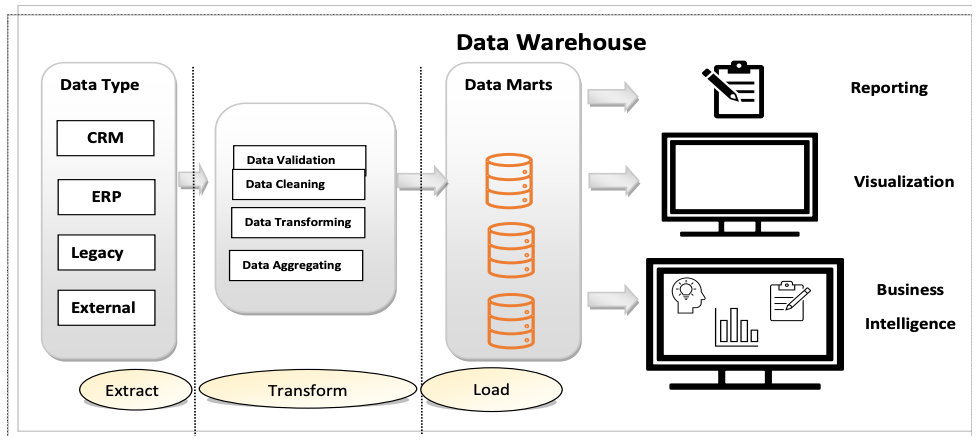
\includegraphics[width=0.7\linewidth]{graphics/dw-architecture.png}
    \caption[Data Warehouse Architektur]{Data Warehouse Architektur (DW).\footnotemark}
    \label{fig:DataWarehouse-Architecture}
    \end{figure}
    \footnotetext{Enthalten in: \cite{10020719}, p. 389}

\ac{DL}s wurden von \cite{dixonPentahoHadoopData2010} als flexible Alternative zu \ac{DW}s entwickelt, siehe Abbildung \ref{fig:DataLake-Architecture}, um große Mengen an unstrukturierten, semi-strukturierten und strukturierten Daten zu speichern.\footcite[Vgl.][S. 390]{10020719} 
\ac{DL} verzichten auf ein vorab definiertes Schema und speichern Daten in ihrer Rohform, was eine hohe Flexibilität bietet. Daten können nach Bedarf organisiert werden, beispielsweise in „Daten-Teiche“ (Data Ponds) für spezifische Datentypen wie rohe Daten, Anwendungsdaten oder Textdaten.\footcite[Vgl.][S. 390]{10020719} 

Abbildung \ref{fig:DataLake-Architecture} illustriert die grundlegende Architektur eines Data Lakes. Daten unterschiedlicher Typen (strukturiert, semi-strukturiert und unstrukturiert) werden extrahiert und geladen, bevor sie in Big Data Systemen wie Hadoop oder SQL/NoSQL-Datenbanken verarbeitet werden. Anschließend durchlaufen sie Prozesse wie die Datenvorbereitung, das Metadatenmanagement und die Governance. Diese Schritte gewährleisten eine effiziente Verwaltung und Bereitstellung der Daten für Analysen und Machine-Learning-Anwendungen.

Diese Strukturierung erleichtert die Handhabung großer Datenmengen, doch Data Lakes stehen vor Herausforderungen wie mangelnder Datenqualität und der Gefahr von „Data Swamps“, in denen unorganisierte und schwer auffindbare Daten die Effektivität einschränken.\footcite[Vgl.][S. 46 ff.]{inmonDataLakeArchitecture2016} 

\begin{figure}[H]\label{fig:DataLake-Architecture}
    \centering
    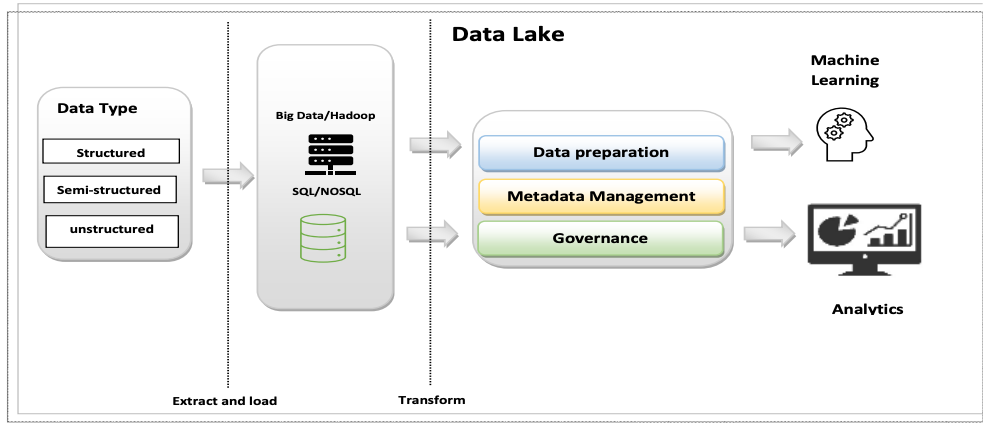
\includegraphics[width=0.7\linewidth]{graphics/dl-architecture.png}
    \caption[Data Lake Architektur]{Data Lake Architektur (DL).\footnotemark}
    \label{fig:DataLake-Architecture}
    \end{figure}
    \footnotetext{Enthalten in: \cite{10020719}, p. 389} 

\section{Definition und Beschreibung von einem Data Lakehouse}
Um die Stärken von \ac{DW}s und \ac{DL}s zu vereinen, wurde die \ac{LH}-Architektur entwickelt. Diese kombiniert die skalierbare, flexible Speicherfähigkeit von \ac{DL}s mit den strukturierten und integrierten Analysefunktionen von \ac{DW}s.\footcite[Vgl.][S. 391]{10020719}

\cite{armbrustLakehouseNewGeneration2021} definiert ein \ac{LH} als ein Datenmanagementsystem, das kostengünstigen, direkt zugänglichen Speicher mit den traditionellen Verwaltungs- und Leistungsmerkmalen eines analytischen \ac{DBMS} kombiniert.\footcite[Vgl.][S. 3]{armbrustLakehouseNewGeneration2021} 
Zu diesen Merkmalen zählen \ac{ACID}-Transaktionen, Datenversionierung, Auditierung, Indexierung, Caching und Abfrageoptimierung.

Ein \ac{LH} bietet eine kostengünstige Speicherung in einem offenen Format, das von verschiedenen Systemen zugänglich ist, während leistungsstarke Verwaltungs- und Optimierungsfunktionen bereitgestellt werden. Die Architektur ist besonders geeignet für Cloud-Umgebungen mit getrennter Verarbeitung und Speicherung.\footcite[Vgl.][S. 3]{armbrustLakehouseNewGeneration2021}
Anwendungen wie \ac{ML}-Modelle können flexibel auf separaten Rechenknoten ausgeführt werden, während sie auf denselben Speicher zugreifen. Gleichzeitig ist auch die Implementierung in lokalen Speicherumgebungen wie \ac{HDFS} möglich.\footcite[Vgl.][S. 3]{armbrustLakehouseNewGeneration2021} 

Ein zentraler Aspekt der \ac{LH}-Architektur ist die Nutzung moderner technologischer Ansätze, die flexible Datenzugänglichkeit mit leistungsstarker Abfrage- und Analyseoptimierung kombinieren. Diese hybride Lösung vereint die Vorteile von \ac{DL}s und \ac{DW}s. Offene Speicherformate wie Apache Parquet oder Delta Lake sowie Cloud-Objektspeicher wie Amazon S3 oder MinIO bilden dabei die Grundlage.\footcite[Vgl.][S. 6]{mazumdarDataLakehouseData2023}

Im Gegensatz zu herkömmlichen \ac{DW}s, die Rechenleistung und Speicher eng koppeln und dadurch in ihrer Skalierbarkeit eingeschränkt sind, entkoppeln Lakehouses diese Komponenten. Dadurch können Abfragen unabhängig von der Datenhaltung in separaten Engines verarbeitet werden, was verteilte Abfragen über verschiedene Datenquellen ermöglicht.\footcite[Vgl.][S. 2]{armbrustLakehouseNewGeneration2021}
Zudem vermeiden \ac{LH} redundante \ac{ETL}-Prozesse und physische Datenkopien, indem sie direkt auf semi-strukturierte Speicher wie S3-Objektspeicher zugreifen.\footcite[Vgl.][S. 2]{armbrustLakehouseNewGeneration2021}

Die Konsistenz der Daten wird durch Metadatenkataloge wie Apache Iceberg gewährleistet, die \ac{ACID}-Transaktionen ermöglichen.\footcite[Vgl.][S. 2]{armbrustLakehouseNewGeneration2021} Optimierungen wie Indexerstellung und effiziente Datenlayouts erhöhen die Abfragegeschwindigkeit erheblich. Dank dieser Eigenschaften etabliert sich die \ac{LH}-Architektur zunehmend als Standard für die Verarbeitung großer Datenmengen.\footcite[Vgl.][S. 2]{armbrustLakehouseNewGeneration2021}

Abbildung \ref{fig:DataLakehouse-Architecture} zeigt den Aufbau eines \ac{LH}. Die Architektur umfasst eine Extraction- und Ingestion-Schicht, die Daten aus verschiedenen Quellen extrahiert und verarbeitet. Im \ac{DL} werden die Daten zunächst in der Landing/Stage Area in ihrer Rohform gespeichert und in der Foundation Area weiter aufbereitet. Anschließend werden sie in das \ac{DW}-Modell überführt, das aus der Base Layer für konsistente Datenspeicherung und der Performance- und Analytics-Layer für schnelle Abfragen, Berichte und Analysen besteht.

\begin{figure}[htb]
    \centering
    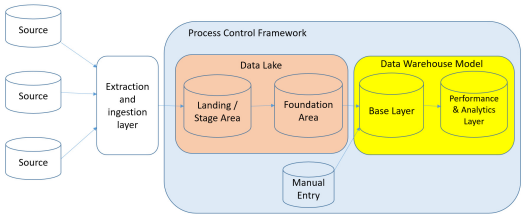
\includegraphics[width=0.7\linewidth]{graphics/lh-architecture.png}
    \caption[Data Lakehouse Architektur]{Data Lakehouse Architektur (LH).\footnotemark}
    \label{fig:DataLakehouse-Architecture} 
    \end{figure}
    \footnotetext{Enthalten in: \cite{d.orescaninDataLakehouseNovel2021}, p. 1243} 

Im Rahmen dieser Arbeit wird die theoretische Grundlage der \ac{LH}-Architektur durch eine praxisorientierte Open Source Umsetzung aufgezeigt. Die einzelnen Komponenten der Architektur werden mithilfe von Containern realisiert. MinIO fungiert als Objektspeicher für Daten im Delta- und Parquetformat, während Apache Spark die Zerlegung der Beispieldaten in Delta-Tabellen und deren Speicherung übernimmt. Für die Verarbeitung und Analyse der Daten werden DuckDB, Pandas und Ibis verwendet. Die Ergebnisse werden in Apache Superset visualisiert, das Dashboards und Diagramme erstellt, um die analysierten Daten übersichtlich darzustellen.

Die Zerlegung und Speicherung der Daten in MinIO bildet die Extraction- und Ingestion-Schicht, während die Foundation Area durch die Datenaufbereitung und Analysen mit DuckDB und Ibis umgesetzt wird. Die Performance- und Analytics-Layer wird durch die Visualisierung in Superset realisiert. Diese Implementierung demonstriert die Flexibilität, Skalierbarkeit und Effizienz der Lakehouse-Architektur in einer Open-Source-Umgebung.

Die \ac{LH} Architektur wird durch ein Process-Control-Framework gesteuert, das eine konsistente Datenverwaltung sicherstellt. Zusätzlich ermöglicht die manuelle Eingabe die Integration spezifischer Daten. Dadurch können \ac{LH}-Systeme komplexe Abfragen und Analysen effizient unterstützen und sind besonders geeignet für Anwendungen wie \ac{ML} und Analytics. Trotz ihrer zahlreichen Vorteile erfordern \ac{LH}-Architekturen eine sorgfältige Integration der Speicher- und Rechenkomponenten sowie eine Optimierung der Abfragen und Datenformate. Technologien wie Delta Lake, Apache Parquet und Metadatenkataloge wie Apache Iceberg spielen hierbei eine zentrale Rolle.\footcite[Vgl.][S. 6]{mazumdarDataLakehouseData2023}